\documentclass[final]{beamer}
\usepackage{hyperref,xspace,graphicx,microtype,minted,multicol,mflogo,enumerate,mathtools,hologo}
\usepackage[brazil]{babel}

\usetheme[sectionpage=none,numbering=none]{metropolis}
\beamertemplatenavigationsymbolsempty

\newcommand{\filename}[1]{\texttt{#1}}
\newcommand{\code}[1]{\texttt{#1}}

\title{Introdução ao \LaTeX\ no SciELO}
\author{Rafael Beraldo}
\date{13 e 14 de junho de 2017}

\begin{document}
\maketitle
%% História %%%%%%%%%%%%%
\section{História}

\begin{frame}[plain]
  \begin{figure}[h]
    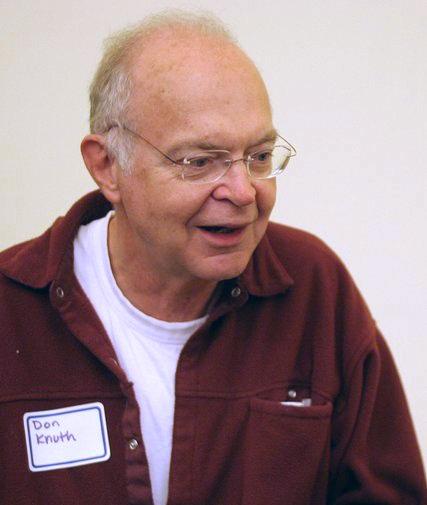
\includegraphics[scale=.5]{imagens/knuth}
    \caption{Donald Knuth em 2005}
  \end{figure}
\end{frame}

\begin{frame}[plain]
  \hspace*{-11.5mm}
  \begin{centering}
    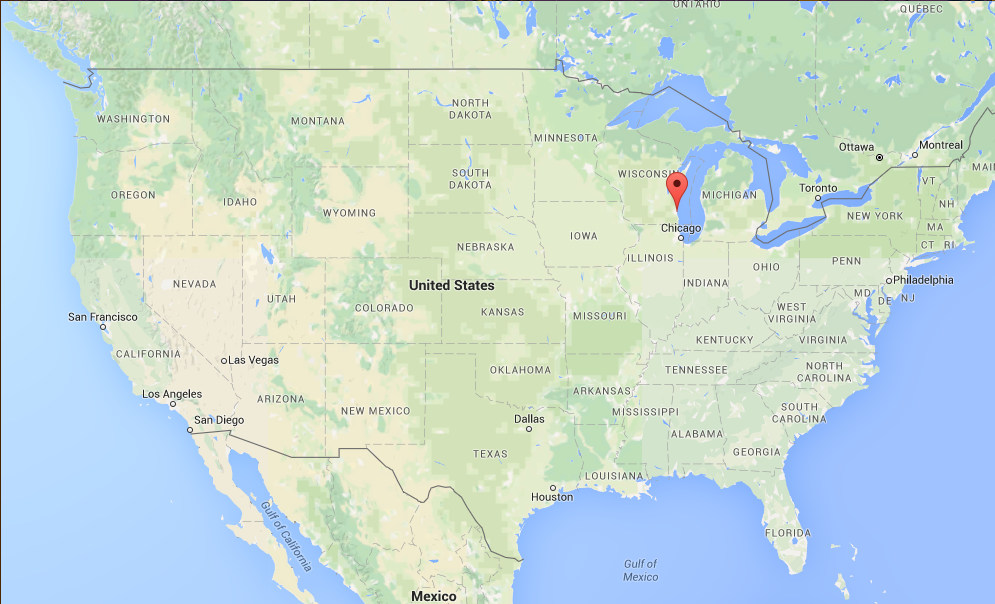
\includegraphics[width=\pagewidth]{imagens/milwaukee}
  \end{centering}
\end{frame}

\begin{frame}
  \frametitle{História do LaTeX}
  \LARGE
  \only<1>{O pai de Knuth\\ tinha uma editora}
  \only<2>{1977: segunda edição do segundo volume de \emph{The Art of Computer
  Programming}}
  \only<3>{\textsc{ascii} não foi projetado\\ com livros em mente}
  \only<4>{\TeX: tau epsilon chi}
\end{frame}

\begin{frame}
  \large
  \begin{quote}
    The purpose of this pronunciation exercise is to remind you that \TeX\ is
    primarily concerned with high-quality technical manuscripts: Its emphasis
    is on art and technology, as in the underlying Greek word. If you merely
    want to produce a passably good document—something acceptable and basically
    readable but not really beautiful—a simpler system will usually suffice.
    With \TeX\ the goal is to produce the finest quality; this requires more
    attention to detail, but you will not find it much harder to go the extra
    distance, and you’ll be able to take special pride in the finished
    product.\hfill (Donald Knuth, \emph{\TeX book})
  \end{quote}
\end{frame}

\begin{frame}
  \frametitle{História do LaTeX}
  \LARGE
  \LaTeX: 1985
\end{frame}

\begin{frame}[plain]
  \begin{figure}[h]
    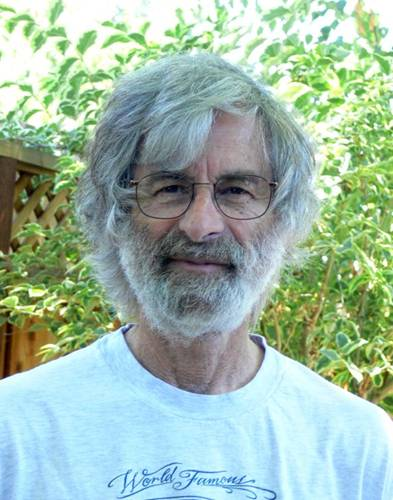
\includegraphics[scale=.5]{imagens/lamport}
    \caption{Leslie Lamport}
  \end{figure}
\end{frame}

% LaTeX: uma linguagem de marcação %%%%%%%%%%%%%%
\section[\LaTeX: uma linguagem de marcação]{Linguagem de marcação}

% O LaTeX é uma linguagem de marcação de texto, ou markup
\begin{frame}
  \frametitle{\LaTeX: uma linguagem de marcação}
  \LARGE
  \only<1>{\LaTeX{} é uma linguagem de \emph{markup}}
  \only<2>{Você \emph{declara} o documento}
  \only<3>{O programa segue as instruções}
  \only<4>{Assim como em \textsc{html},\\ o arquivo fonte é renderizado}
  \only<5>{Comandos são semânticos}
\end{frame}

% Se os comandos são semânticos, devem ser fáceis de interpretar. O que os
% comandos abaixo significam?
\begin{frame}[fragile]
  \frametitle{\LaTeX: uma linguagem de marcação}
  \begin{minted}[autogobble,fontsize=\LARGE,breaklines]{latex}
    \tableofcontents

    \section{Introdução}
  \end{minted}
\end{frame}

% Arquivos .tex não contém formatação; são texto plano.
\begin{frame}
  \frametitle{\LaTeX: uma linguagem de marcação}
  \LARGE
  \code{.tex} são arquivos de texto plano
\end{frame}

% Exemplo de artigo %%%%%%%%%%%%%%
\section{Exemplo de artigo}

% Vejamos nosso primeiro artigo em LaTeX.
\begin{frame}
  \frametitle{Exemplo de artigo}
  \Huge
  Vejamos \filename{exemplo/artigo.tex}
\end{frame}

% Comandos %%%%%%%%%%%%%%
% Sintaxe dos comandos LaTeX
\begin{frame}[standout]
  \Huge
  Comandos
\end{frame}

% Comandos simples não têm argumentos
\begin{frame}[fragile]
  \frametitle{Comandos simples}
  \begin{minted}[autogobble,fontsize=\huge,breaklines]{latex}
    \tableofcontents
  \end{minted}
\end{frame}

% Comandos simples e espaço em branco
\begin{frame}[fragile]
  \frametitle{Comandos simples e espaço em branco}
  \begin{minted}[autogobble,fontsize=\normalsize,breaklines]{latex}
    \tableofcontents Embora isso funcione, o próximo exemplo ganha mais pontos por estilo e ajuda na leitura do código. Por quê?
  \end{minted}
\end{frame}

\begin{frame}[fragile]
  \frametitle{Comandos simples e espaço em branco}
  \begin{minted}[autogobble,fontsize=\normalsize,breaklines]{latex}
    \tableofcontents
    Esse exemplo é melhor, mas como espaço em branco não faz diferença, talvez valesse a pena colocar mais uma linha entre o parágrafo e o comando.
  \end{minted}
\end{frame}

% Comandos com argumentos
\begin{frame}[fragile]
  \frametitle{Comandos com argumento}
  \begin{minted}[autogobble,fontsize=\normalsize,breaklines]{latex}
    \section{Introdução}\label{introducao}Este exemplo funciona, mas o código não é muito legível. O resultado será perfeito, entretanto.
  \end{minted}
\end{frame}

% Voltemos ao exemplo para demonstrar
\begin{frame}[standout]
  \Huge
  \filename{exemplo/artigo.tex}
\end{frame}

% Espaço em branco %%%%%%%%%%%%%%
\begin{frame}[standout]
  \Huge
  Espaço em branco
\end{frame}

% Espaços em branco são condensados
\begin{frame}[fragile]
  \frametitle{Espaços em branco}
  \begin{minted}[autogobble,fontsize=\normalsize,breaklines]{latex}
    \section      {Introdução}
        \label{introducao}

        Este exemplo funciona, mas o código não é
     muito legível.  O resultado será perfeito, entretanto.
  \end{minted}
\end{frame}

% Voltemos ao exemplo para aprender mais sobre espaços em branco e como usá-lo
% de maneira a deixar seu código mais legível.
\begin{frame}[standout]
  \Huge
  \filename{exemplo/artigo.tex}
\end{frame}

% Vamos resolver nosso primeiro exercício e compilar o arquivo. Haverá um
% problema bem claro.
\begin{frame}[standout]
  \Huge
  \filename{exercicios/espaco-branco.tex}
\end{frame}

% Símbolos especiais %%%%%%%%%%%%%%
\begin{frame}[standout]
  \Huge
  Símbolos especiais
\end{frame}

% Aspas
\begin{frame}[fragile]
  \frametitle{Aspas}
  \begin{minted}[autogobble,fontsize=\LARGE,breaklines]{latex}
    ``Devemos abrir aspas com dois acentos graves e fechar com duas aspas
    simples.''
  \end{minted}
\end{frame}

% Traços
\begin{frame}[fragile]
  \frametitle{Hífen, travessão e meia-risca}
  \begin{minted}[autogobble,fontsize=\LARGE,breaklines]{latex}
    Leve um guarda-chuva --- ouvi na rádio que pode chover entre 10h--13h.
  \end{minted}
\end{frame}

% Os símbolos a seguir são especiais e devem ser escapados:
\begin{frame}[fragile]
  \frametitle{Caracteres reservados}
  \begin{minted}[autogobble,fontsize=\LARGE,breaklines]{latex}
    # $ % ^ & _ { } ~ \

    \# \$ \% \^{} \& \_ \{ \} \~{} \textbackslash
  \end{minted}
\end{frame}

% Resolver o exercício
\begin{frame}[standout]
  \Huge
  \filename{exercicios/caracteres\-reservados.tex}
\end{frame}

% Preambulo do documento %%%%%%%%%%%%%%
\begin{frame}[standout]
  \Huge
  Preâmbulo do documento
\end{frame}

% Dar uma olhada no arquivo. Ensinar a distinção entre o preâmbulo e o corpo do
% documento.
\begin{frame}
  \frametitle{Preâmbulo do documento}
  \LARGE
  Documentos \LaTeX: preâmbulo e corpo
\end{frame}

\begin{frame}[fragile]
  \frametitle{Preâmbulo do documento}
  \LARGE
  \begin{minted}[autogobble,fontsize=\large,breaklines]{latex}
  \documentclass[11pt,a4paper,oneside]{article}
  \end{minted}
\end{frame}

% Explicar as opções da classe article que escolhi
\begin{frame}[fragile]
  \frametitle{Preâmbulo do documento}
  \huge
  Classes comuns:
  \begin{multicols}{2}
    \begin{itemize}
      \item\code{article}
      \item\code{report}
      \item\code{book}
      \item\code{letter}
      \item\code{memoir}
      \item\code{beamer}
  \end{itemize}
\end{multicols}
\end{frame}

% Vejamos quais são as opções de classe mais comuns
\begin{frame}
  \frametitle{Preâmbulo do documento}
  \LARGE
  Opções de classe comuns:
  \begin{itemize}
    \only<1>{\item \code{10pt, 11pt, 12pt}}
    \only<1>{\item \code{a4paper, a5paper, letterpaper, …}}
    \only<1>{\item \code{fleqn}}
    \only<2>{\item \code{leqno}}
    \only<2>{\item \code{titlepage, notitlepage}}
    \only<2>{\item \code{twocolumn}}
    \only<2>{\item \code{twoside, oneside}}
    \only<3>{\item \code{landscape}}
    \only<3>{\item \code{openright, openany}}
    \only<3>{\item \code{draft}}
  \end{itemize}
\end{frame}

\begin{frame}
  \frametitle{Preâmbulo do documento}
  \huge
  Vejamos \filename{exemplos/artigo.tex}
\end{frame}

\begin{frame}
  \frametitle{Preâmbulo do documento}
  \huge
  Resolver \filename{exercicios/meu\-artigo.tex}
\end{frame}

% Corpo do documento %%%%%%%%%%%%%%
\section{Corpo do documento}

% O corpo do documento
\begin{frame}[fragile]
  \frametitle{Corpo do documento}
  \begin{minted}[autogobble,fontsize=\Large,breaklines]{latex}
    \begin{document}
     …
    \end{document}
  \end{minted}
\end{frame}

% Divisões do documento
\begin{frame}[fragile]
  \frametitle{Corpo do documento: divisões do documento}
  \large
  \begin{multicols}{2}
    \begin{itemize}
      \item\latexcode{\part} (-1)
      \item\latexcode{\chapter} (0)
      \item\latexcode{\section} (1)
      \item\latexcode{\subsection} (2)
      \item\latexcode{\subsubsection} (3)
      \item\latexcode{\paragraph} (4)
      \item\latexcode{\subparagraph} (5)
    \end{itemize}
  \end{multicols}
\end{frame}

% Profundidade
\begin{frame}[fragile]
  \frametitle{Corpo do documento: profundidade das divisões}
  \begin{minted}[autogobble,fontsize=\Large,breaklines]{latex}
  \setcounter{secnumdepth}{3}
  \setcounter{tocdepth}{3}
  \end{minted}
\end{frame}

% Comandos estrelados para controlar numeração e o que vai no sumário
\begin{frame}[fragile]
  \frametitle{Corpo do documento: comandos estrelados}
  \begin{minted}[autogobble,fontsize=\large,breaklines]{latex}
  \section*{Esta seção não terá numeração nem aparecerá no sumário}
  \end{minted}
\end{frame}

% Sintaxe para controlar título que vai no sumário
\begin{frame}[fragile]
  \frametitle{Corpo do documento: controlar texto do sumário}
  \begin{minted}[autogobble,fontsize=\large,breaklines]{latex}
  \section[Seção muito longa]{Seção muito longa: provavelmente não ficará muito boa no sumário.}
  \end{minted}
\end{frame}

\begin{frame}
  \frametitle{Corpo do documento: parágrafos}
  \LARGE
  Parágrafos são separados\\
  por linhas em branco
\end{frame}

\begin{frame}[fragile]
  \frametitle{Corpo do documento: espaçamento entre parágrafos}
  \begin{minted}[autogobble,fontsize=\Large,breaklines]{latex}
  \setlength{\parskip}{1cm}
  \setlength{\parskip}{1cm plus4mm minus3mm}
  \end{minted}
\end{frame}

\begin{frame}
  \frametitle{Corpo do documento: indentação}
  \LARGE
  Pacote \code{indentfirst}
\end{frame}

\begin{frame}
  \frametitle{Corpo do documento}
  \huge
  Vejamos \filename{exemplo/artigo.tex}
\end{frame}

\begin{frame}
  \frametitle{Corpo do documento}
  \huge
  Resolver \filename{exercicios/meu\-artigo.tex}
\end{frame}

%
% pacotes.tex
%
% Rafael Beraldo <rberaldo@cabaladada.org>
% Workshop de LaTeX do SciELO
%
% Problema: ao compilar este documento, os acentos não aparecem no PDF.
% Adicione o pacote polyglossia após a linha 13, configure o idioma português e
% compile.
%

\documentclass{article}
\begin{document}
  Muito além, nos confins inexplorados da região mais brega da
  Borda Ocidental desta Galáxia, há um pequeno sol amarelo e esquecido.

  Girando em torno deste sol, a uma distância de cerca de 148~milhões de
  quilômetros, há um planetinha verde-azulado absolutamente insignificante.
\end{document}

%
% fontes.tex
%
% Rafael Beraldo <rberaldo@cabaladada.org>
% Workshop de LaTeX do Opensanca
%
% Demonstra:
% - Inserção de diacríticos antes e hoje
% - Tamanhos e estilos de fonte
% - Como selecionar outras fontes
%

\documentclass[11pt,a4paper,oneside]{article}
% O pacote fontspec usa a codificação TU (TeX Unicode) por padrão:
\usepackage{fontspec}
% Selecionar fontes:
% \setmainfont{Linux Libertine}
%
% Selecionar a língua:
\usepackage{polyglossia}
  \setdefaultlanguage{brazil}

\title{Fontes no \LaTeX}
\author{Rafael Beraldo}

\begin{document}
\frenchspacing

\maketitle

\section{Codificações}

Este é um parágrafo cheio de acentos e palavras. Antigamente, seria necessário
escrever “tip\'{o}grafos trabalhar\~{a}o”, mas hoje é fácil adicionar símbolos
Unicode diretamente, como esta seta: →

\section{Fontes e suas famílias}

No passado, fontes não costumavam ter \emph{tantos} estilos. Tipógrafos
compunham livros inteiros com apenas um tipo e um tamanho. Hoje, temos uma
miríade de possibilidades. Empregá-las com sabedoria e, talvez, um pouco de
parcimônia não são más ideias.

As fontes que usamos comumente contam com tipos como:

\begin{itemize}
  \item O \emph{itálico,} geralmente usado para enfatizar ideias.
  \item O \textbf{negrito}, ou \textbf{bold}, muitas vezes usado para chamar a
    atenção do leitor.
  \item Os \textsc{versaletes}, que são letras em estilo de maiúscula, mas com
    a mesma altura do corpo da fonte. Uma boa ideia é usá-los em siglas, como
    \textsc{ibge}, \textsc{bc}, 3~\textsc{am} etc. Em nomes próprios e
    acrônimos geográficos, geralmente usamos maiúsculas como JRR Tolkien.
  \item Os \texttt{tipos monoespaçados} são ótimos para dar exemplos de
    código-fonte ou nomes de arquivos, como \texttt{fontes.tex}.
\end{itemize}

\section{Tamanhos de fontes}

Como já vimos, certos comandos como \verb+\section+ e \verb+chapter+ escolhem o
tamanho e espaçamento adequados para que nosso texto pareça organizado e
fluido. Essas decisões são tomadas pelos designers das classes que usamos e
baseadas em \textbf{escalas} tipográficas. Nas raras ocasiões em que precisamos
\footnotesize diminuir \Large ou aumentar \normalsize nosso texto, temos os seguintes
comandos à nossa disposição:

\begin{itemize}
  \item\verb+\tiny+
  \item\verb+\scriptsize+
  \item\verb+\footnotesize+
  \item\verb+\small+
  \item\verb+\normalsize+
  \item\verb+\large+
  \item\verb+\Large+
  \item\verb+\LARGE+
  \item\verb+\huge+
  \item\verb+\Huge+
\end{itemize}

{\Large É possível conter nosso texto entre duas chaves} para que apenas uma
seção seja afetada pelo comando de tamanho.

\end{document}

% Layouts de página %%%%%%%%%%%%%%
\begin{frame}[standout]
  \Huge
  Layouts de página
\end{frame}

% Vamos mudar a opção de classe de onecolumn para twocolumn e carregar o pacote
% showframe.
\begin{frame}
  \frametitle{Layouts de página}
  \Large
  \only<1>{Copiar solução de \filename{exercicio/sonhos-noite\-verao.tex} em
  \filename{exemplos/layouts-pagina.tex}}
  \huge
  \only<2>{Mudar para \code{twocolumn}, carregar o pacote \code{showframe}}
\end{frame}

% Na folha A4, apenas uma coluna coluna de texto é difícil de ler com margens
% curtas. Mas usar margens grandes desperdiça papel.
\begin{frame}
  \frametitle{Layouts de página}
  \huge
  \code{onecolumn}: margens grandes demais

  \code{twocolumn}: nem sempre podemos
\end{frame}

% Soluções para o problema do tamanho da coluna de texto vs margens
\begin{frame}
  \frametitle{Layouts de página}
  \huge
  Soluções:
  \begin{itemize}
    \only<1>{\item Colunas}
    \only<2>{\item \code{fullpage}}
    \only<3>{\item \code{fullpage} e entrelinhas maiores}
  \end{itemize}
\end{frame}

% Se decidirmos usar o pacote fullpage, é uma boa ideia aumentar o espaçamento
% entre as linhas.
\begin{frame}
  \frametitle{Layouts de página}
  \huge
  Pacote \code{setspace}:

  \begin{itemize}
    \item \code{\textbackslash singlespacing}
    \item \code{\textbackslash onehalfspacing}
    \item \code{\textbackslash doublespacing}
  \end{itemize}
\end{frame}

% Outro fator que influencia o layout da página é seu estilo. Estes são os três
% comandos básicos e estilos que podemos escolher.
\begin{frame}
  \frametitle{Layouts de página}
  \huge
  \code{\textbackslash pagestyle} e \code{\textbackslash thispagestyle}

  \begin{itemize}
    \item \code{empty}
    \item \code{plain}
    \item \code{headings}
  \end{itemize}
\end{frame}

% Outro fator que influencia o layout da página é seu estilo. Estes são os três
% comandos básicos e estilos que podemos escolher.
\begin{frame}
  \frametitle{Layouts de página}
  \huge
  Demonstração em \filename{exemplos/layouts\-pagina.tex}
\end{frame}

% Exercício: faremos um certificado de conclusão do curso
\begin{frame}
  \frametitle{Layouts de página}
  \Huge
  Vamos fazer um certificado
\end{frame}

% Uma certificado incompleto
\begin{frame}[plain]

  {\huge\textbf{SciELO}}\\[2em]
  {\LARGE\textsc{Certificado}}

  \noindent Certificamos que José João da Silva participou de um curso em nosso
  grupo no dia 28 de maio de 1999 e está qualificado para editar textos em
  \LaTeX.

  \vfill
  \emph{Os Organizadores}\\
  \emph{SciELO}

\end{frame}

% Começar nosso certificado de conclusão de curso
\begin{frame}
  \frametitle{Layouts de página}
  \huge
  Resolver \filename{exercicios/certificado.tex}
\end{frame}

% Posição do texto %%%%%%%%%%%%%%
\section{Posição do texto}

% Nosso certificado pode ter ficado legal, mas poderia ser melhor ainda se
% ajustarmos o texto em relação à página.
\begin{frame}
  \frametitle{Posição do texto}
  \LARGE
  Problemas com\\ o certificado?
\end{frame}

% Antes de controlar a posição do texto, temos que entender o que é um
% ambiente.
\begin{frame}[fragile]
  \frametitle{Posição do texto}
  \LARGE
  Ambientes:

  \begin{minted}[autogobble,fontsize=\LARGE,breaklines]{latex}
    \begin{ambiente}
      …
    \end{ambiente}
  \end{minted}
\end{frame}

% Três ambientes para controlar posição.
\begin{frame}[fragile]
  \frametitle{Posição do texto}
  \Large
  Ambientes \code{center}, \code{flushleft} e \code{flushright}

  % Código:
  \begin{minted}[autogobble,fontsize=\Large,breaklines]{latex}
    \begin{center}
      Este texto será centralizado.
    \end{center}
  \end{minted}

  % Resultado:
  \begin{center}
    Este texto será centralizado.
  \end{center}
\end{frame}

% Ainda podemos controlar o espaço dentro de uma linha.
\begin{frame}[fragile]
  \frametitle{Posição do texto}
  \LARGE
  \latexcode{\hspace{comprimento}}
\end{frame}

% Por exemplo, um espaço de 2cm:
\begin{frame}[fragile]
  \frametitle{Posição do texto}
  \LARGE
  \begin{minted}[autogobble,fontsize=\LARGE,breaklines]{latex}
    Frase\hspace{2cm} esticada.
  \end{minted}
  \vspace{1em}

  Frase\hspace{2cm} esticada.
\end{frame}

% O LaTeX aceita uma série de unidades
\begin{frame}[fragile]
  \frametitle{Posição do texto}
  \LARGE
  Unidades que o \LaTeX{} conhece:

  \begin{multicols}{2}
    \begin{itemize}
      \item\code{mm}
      \item\code{cm}
      \item\code{in}
      \item\code{pt}
      \item\code{em}
      \item\code{ex}
      \item\latexcode{\textheight}
      \item\latexcode{\textwidth}
      \item\latexcode{\pageheight}
      \item\latexcode{\pageheight}
    \end{itemize}
  \end{multicols}
\end{frame}

% O comando \hfill preenche todo o espaço disponível
\begin{frame}[fragile]
  \frametitle{Posição do texto}
  \LARGE
  \latexcode{Começo\hfill meio\hfill fim}
  \vspace{1em}

  Começo\hfill meio\hfill fim
\end{frame}

% E, finalmente, existem os comandos \vspace e \hfill
\begin{frame}[fragile]
  \frametitle{Posição do texto}
  \LARGE
  Comandos análogos:

  \latexcode{\vspace{comprimento}}
  \vspace{1em}

  \latexcode{\vfill}
\end{frame}

% Vejamos uma demonstração.
\begin{frame}
  \frametitle{Posição do texto}
  \huge
  Demonstração em \filename{exemplos/posicao\-texto.tex}
\end{frame}

% Sugestão para o visual final do certificado
\begin{frame}[plain]
  \begin{center}
    {\huge\textbf{SciELO}}\\[2em]
    {\LARGE\textsc{Certificado}}
  \end{center}

    \noindent Certificamos que José João da Silva participou de um curso em
    nosso grupo no dia 28 de maio de 1999 e está qualificado para editar textos
    em \LaTeX.

    \vfill
    \begin{flushright}
      \rule{\widthof{\phantom{\emph{Os Organizadores}}}}{.4pt}\\
      \emph{Os Organizadores}\\
      \emph{SciELO}\\
    \end{flushright}
\end{frame}

% Exercício: terminar o certificado que começamos antes
\begin{frame}
  \frametitle{Posição do texto}
  \huge
  Resolver \filename{exercicios/certificado\-posicionado.tex}
\end{frame}

%%
% listas.tex
%
% Workshop de LaTeX do SciELO
%
% Demonstra:
% - Três ambientes para listas: itemize, enumerate e description
% - Sintaxe para listas e listas aninhadas
% - Customização do ambiente enumerate com o pacote enumerate
%

\documentclass[a4paper,oneside]{article}
\usepackage{fontspec}
\usepackage{polyglossia}
  \setdefaultlanguage{brazil}
\usepackage{enumerate}

\begin{document}
\frenchspacing

\section{Listas}

\LaTeX{} vem com três ambientes para criar listas: \texttt{itemize, enumerate}
e \texttt{description}.

% Mudar o tipo de lista para enumerate
\begin{itemize}
  \item O ambiente \texttt{itemize} é geralmente usado para listas cuja ordem
    não é importante.
  \item A numeração que listas do tipo \texttt{enumerate} trazem pode indicar
    os passos necessários para completar uma tarefa, ou sua ordem de
    importância.
  \item A lista do tipo \texttt{description} é excelente para explicar
    conceitos relacionados. Que oportunidade perdida de usá-la!
\end{itemize}

Listas de descrição têm uma sintaxe um pouco diferente:

\begin{description}
  \item[Bit] Abreviação de \emph{binary digit}, um bit pode tomar o valor de~1
    ou~2, apenas.
  \item[Byte] Uma unidade de informação digital que geralmente tem oito bits.
    O~“y” foi escolhido de propósito para evitar que fosse acidentalmente
    confundido com “bit”.
\end{description}

\section{Customizando o ambiente \texttt{enumerate}}

É possível customizar o ambiente \texttt{enumerate} adicionando o pacote
\texttt{enumerate} ao seu preâmbulo. O resultado é que o ambiente aceitará um
argumento na forma de uma string que contém um desses valores: \texttt{A,
a, I, i} ou~\texttt{1}.

% Demonstrar diferentes possibilidades de customização
\begin{enumerate}[A)]
  \item Tales de Mileto
  \item Pitágoras
  \item Xenófanes
  \item Empédocles
  \item Aristóteles
\end{enumerate}
\end{document}

%\input{citacoes-versos}
%% Tabelas %%%%%%%%%%%%%%
\section{Tabelas}

\begin{frame}
  \frametitle{Tabelas}
  \LARGE
  A abordagem é diferente\\
  dos programas WISIWYG.
\end{frame}

% Exemplo simples de tabela com o ambiente tabular
\begin{frame}[fragile]
  \frametitle{Tabelas: exemplo simples}
  \LARGE
  Exemplo do ambiente \code{tabular}:
  \vspace{1em}

  \begin{minipage}{.65\textwidth}
    \begin{minted}[autogobble,fontsize=\Large,breaklines]{latex}
      \begin{tabular}{lcr}
        1 & 2 & 3\\
        4 & 5 & 6\\
        7 & 8 & 9
      \end{tabular}
    \end{minted}
  \end{minipage}
  \hspace{.05\textwidth}
  \begin{minipage}{.25\textwidth}
    \begin{tabular}{lcr}
      1 & 2 & 3\\
      4 & 5 & 6\\
      7 & 8 & 9
    \end{tabular}
  \end{minipage}
\end{frame}

% Com mais alguns detalhes como linhas verticais e horizontais
\begin{frame}[fragile]
  \frametitle{Tabelas: linhas}
  \LARGE
  Linhas horizontais e verticais:
  \vspace{1em}

  \begin{minipage}{.65\textwidth}
    \begin{minted}[autogobble,fontsize=\Large,breaklines]{latex}
      \begin{tabular}{l|c|r}
        \hline
        1 & 2 & 3\\
        4 & 5 & 6\\
        7 & 8 & 9\\
        \hline
      \end{tabular}
    \end{minted}
  \end{minipage}
  \hspace{.05\textwidth}
  \begin{minipage}{.25\textwidth}
    \begin{tabular}{l|c|r}
      \hline
      1 & 2 & 3\\
      4 & 5 & 6\\
      7 & 8 & 9\\
      \hline
    \end{tabular}
  \end{minipage}
\end{frame}

% O espaço em branco deixa o texto respirar e evita a tirania das linhas retas.
% Essa citação do Bringhurst é fantástica.
\begin{frame}
  \frametitle{Tabelas: espaço branco}
  \large
  \begin{quote}
    Assim como o texto, as tabelas ficam canhestras quando abordadas de forma
    puramente técnica. Boas soluções tipográficas não costumam surgir em resposta
    a perguntas do tipo “Como posso enfiar essa quantidade de caracteres naquele
    tanto de espaço?”.\\[1em]

    (Robert Bringhurst, \emph{Elementos do Estilo Tipográfico)}
  \end{quote}
\end{frame}

% Vejamos alguns exemplos
\begin{frame}
  \frametitle{Tabelas: exemplo}
  \Huge
  Vejamos \filename{exemplos/tabelas.tex}
\end{frame}

% Vamos revisar o que aprendemos no exemplo.
\begin{frame}[fragile]
  \frametitle{Tabelas: revisão}
  \LARGE
  Aprendemos:

  \begin{itemize}
    \only<1>{\item \code{tabular}}
    \only<1>{\item tipografia da tabela}
    \only<1>{\item quebras de linhas}
    \only<2>{\item \code{booktabs}}
    \only<2>{\item \latexcode{\multicolumn}}
    \only<2>{\item \code{longtable}}
  \end{itemize}
\end{frame}

% Temos declarado exatamente onde desejamos que a tabela fique, mas essa
% abordagem nem sempre é boa, porque interrompe o fluxo do texto. Vamos
% aprender mais sobre os ambientes do tipo float.
\begin{frame}
  \frametitle{Tabelas: floats}
  \LARGE
  \only<1>{Ambiente \code{tabular} coloca\\ a tabela após o texto}
  \only<2>{Padrão profissional: \emph{floats}}
  \only<3>{Dois floats: \code{table} e \code{figure}}
\end{frame}

% A sintaxe do ambiente table
\begin{frame}[fragile]
  \frametitle{Tabelas: \code{table}}
  \LARGE
  Sintaxe de \code{table}:
  \vspace{1em}

    \begin{minted}[autogobble,fontsize=\LARGE,breaklines]{latex}
      \begin{table}[posição]
        …
      \end{table}
    \end{minted}
\end{frame}

% Exemplo, com os comandos \centering, \caption e \label.
\begin{frame}[fragile]
  \frametitle{Tabelas: \code{table}}
  \large
  Veja a tabela~\ref{tab:numerosUmNove}:
  \vspace{1em}

  \begin{minipage}{.65\textwidth}
    \begin{minted}[autogobble,fontsize=\large,breaklines]{latex}
    \begin{table}
      \centering
      \begin{tabular}{lcr}
      1 & 2 & 3\\
      4 & 5 & 6\\
      7 & 8 & 9
      \end{tabular}
      \caption{Números de 1 a 9}
      \label{tab:numerosUmNove}
    \end{table}
    \end{minted}
  \end{minipage}
  \hspace{.05\textwidth}
  \begin{minipage}{.25\textwidth}
    \begin{table}
      \centering
      \begin{tabular}{lcr}
        1 & 2 & 3\\
        4 & 5 & 6\\
        7 & 8 & 9
      \end{tabular}
      \caption{Números de 1 a 9}
      \label{tab:numerosUmNove}
    \end{table}
  \end{minipage}
\end{frame}

% Voltaremos ao arquivo anterior para brincar com esses conceitos e
% referências cruzadas.
\begin{frame}
  \frametitle{Tabelas: exemplos de \code{table}}
  \Huge
  Voltemos à \filename{exemplos/tabelas.tex}
\end{frame}

% Exercício: uma tabela do zero, usando o ambiente table e referenciando a
% tabela num parágrafo anterior.
\begin{frame}
  \frametitle{Tabelas: exercício}
  \Huge
  Resolver: \filename{exercicios/robos.tex}
\end{frame}

\begin{frame}
  \frametitle{Tabelas: ferramentas}
  \Huge
  Mais recursos em \filename{conteudo.md}
\end{frame}

%%
% imagens.tex
%
% Workshop de LaTeX do SciELO
%
% Demonstra:
% - Como incluir gráficos com o pacote graphicx
% - Controlar o tamanho e escala dos gráficos
% - O ambiente figure
% - O ambiente minipage e seus usos
%

\documentclass[a4paper,oneside]{article}
\usepackage{fontspec}
\usepackage{polyglossia}
  \setdefaultlanguage{brazil}
\usepackage{graphicx}

\begin{document}
\frenchspacing

% Informação e imagem encontrados na Wikipédia em:
% https://en.wikipedia.org/wiki/Alpha_Centauri
\section{Nosso vizinhos}

Na figura~\ref{fig:estrelas}, podemos ver nossos vizinhos mais próximos, por
assim dizer. A estrela circulada é Proxima Centauri, uma pequena anã vermelha,
que pode estar ligada gravitacionalmente às outras duas estrelas. A olho nu, as
duas estrelas parecem uma só.

% Brincar os as opções de posicionamento do figure e de tamanho do
% \includegraphics. Ensinar o ambiente minipage, e a técnica de colocar dois
% minipages dentro de um figure para colocar uma imagem ao lado da outra.
\begin{figure}[h]
  \centering
  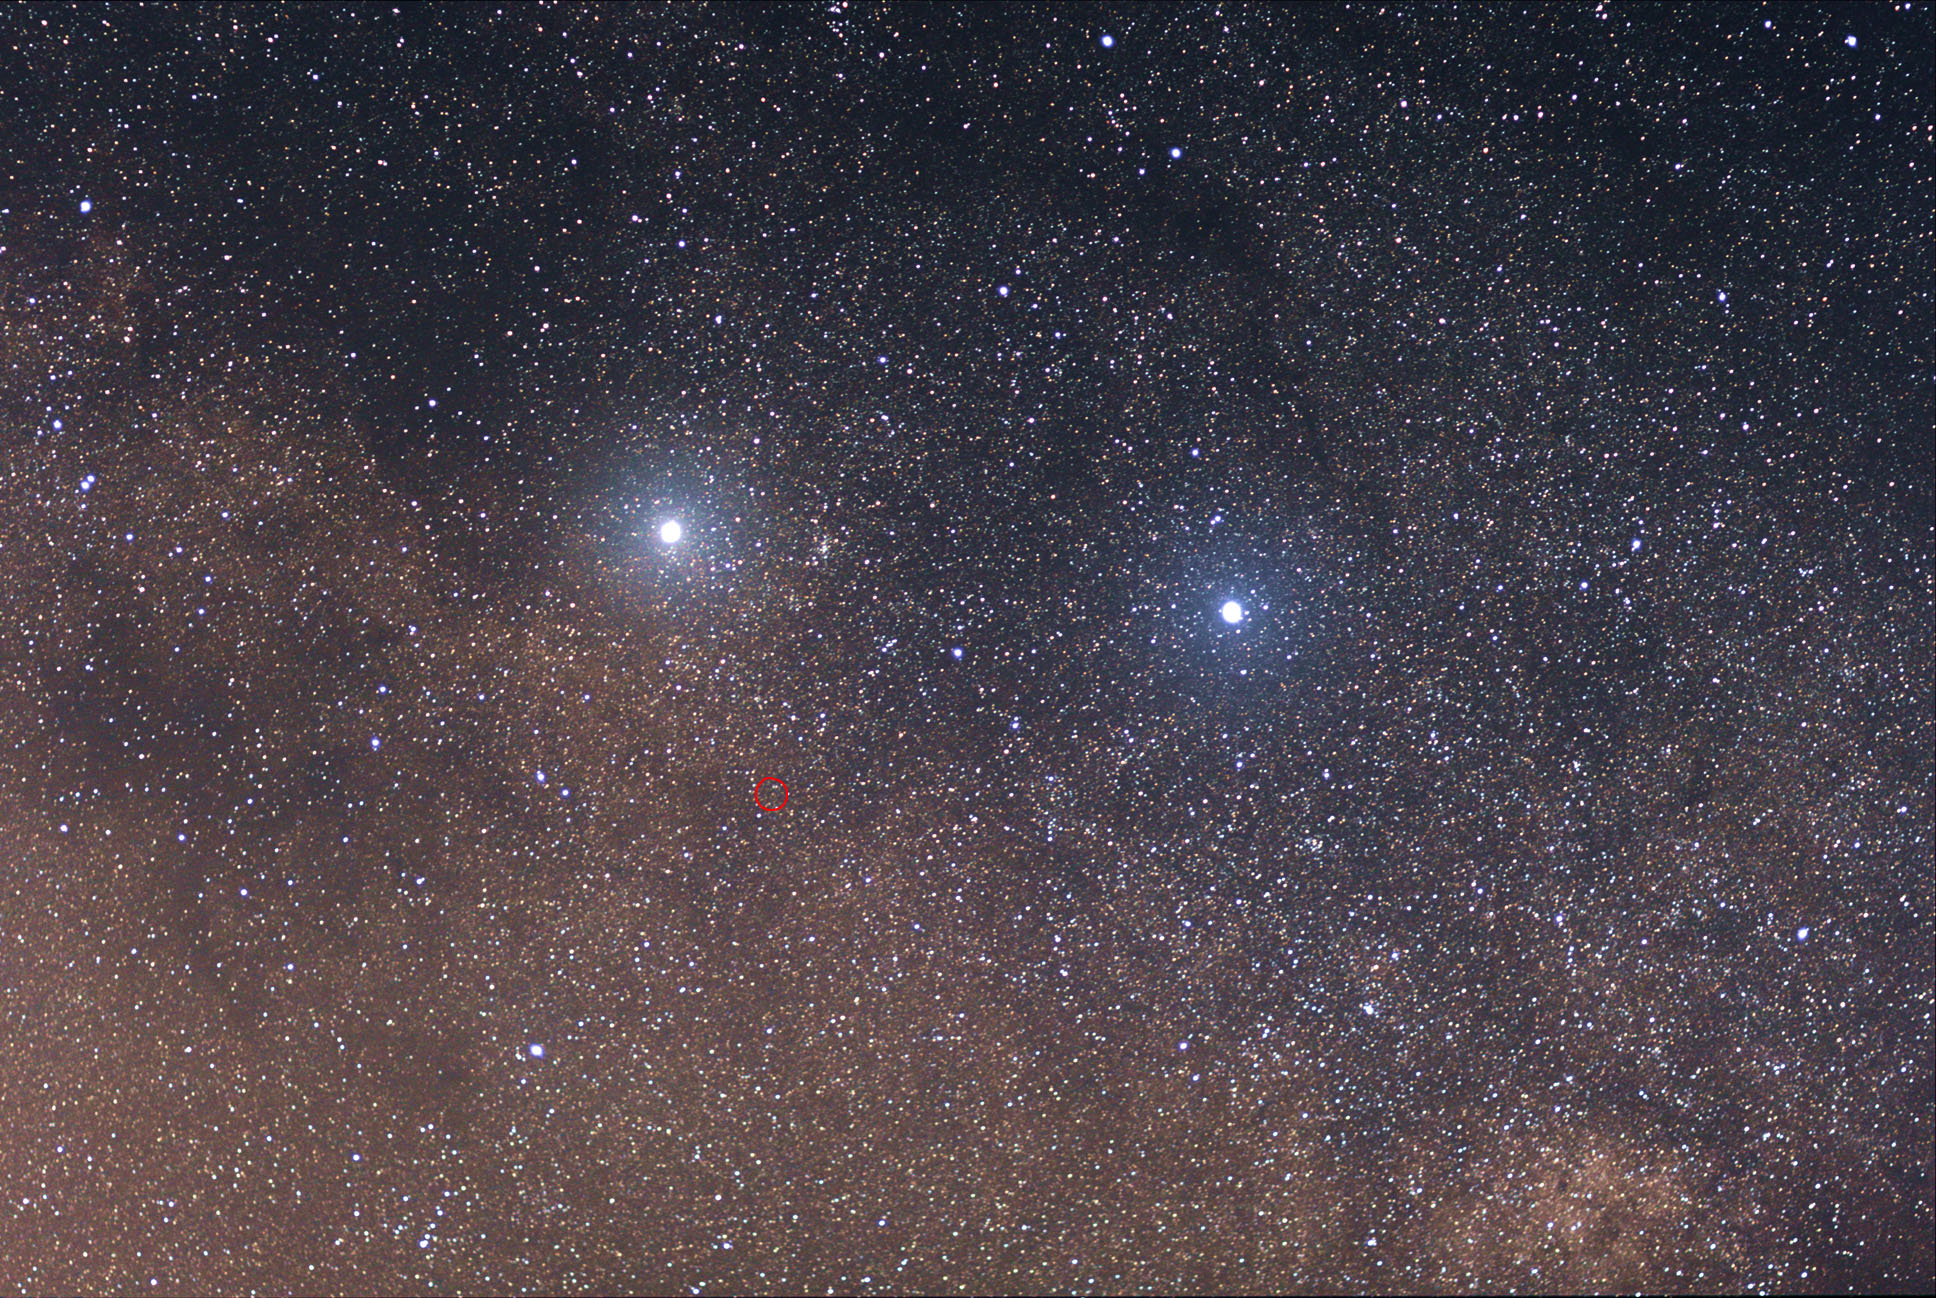
\includegraphics[width=\textwidth]{imagens/alpha-beta-proxima-centauri}
  \caption{Alpha Centauri e Beta Centauri, com Proxima circulada}
  \label{fig:estrelas}
\end{figure}
\end{document}

%% Matemática %%%%%%%%%%%%%%
\section{Matemática}

% Até agora, estávamos no modo de texto. No modo de matemática, o modo como o
% LaTeX interpreta o que escrever é diferente. Além disso, o modo de matemática
% é dividido em dois tipos: inline e displayed
\begin{frame}
  \frametitle{Matemática: modos do \LaTeX}
  \LARGE
  \only<1>{Modo de texto vs.\\ modo de matemática}
  \only<2>{Modo de matemática:\\ \emph{inline} e \emph{displayed}}
\end{frame}

% Existem três ambientes para acessar o modo de matemática.
\begin{frame}[fragile]
  \frametitle{Matemática: ambientes}
  \LARGE
  Três ambientes:\\

  \only<1>{\mintinline{latex}{math} ou \mintinline{latex}{\( … \)}}
  \only<2>{\mintinline{latex}{displaymath} ou \mintinline{latex}{\[ … \]}}
  \only<3>{\mintinline{latex}{equation}}
\end{frame}

% Há uma infinidade de comandos, pacotes e técnicas para aprender. Cobriremos o
% básico.
\begin{frame}
  \frametitle{Matemática}
  \LARGE
  Cobriremos o básico!

  Mais em \url{www.en.wikibooks.org/wiki/LaTEX/Mathematics}
\end{frame}

% Símbolos em modo matemático
\begin{frame}[fragile]
  \frametitle{Matemática: símbolos}
  \LARGE
  \mintinline{latex}{2 \times 2 = 4}
  \hfill
  \( 2 \times 2 = 4 \)
\end{frame}

% Alfabeto grego
\begin{frame}[fragile]
  \frametitle{Matemática: alfabeta grego}
  \LARGE
  \mintinline{latex}{\alpha, \beta, \pi}
  \hfill
  \( \alpha, \beta, \pi \)
\end{frame}

% Operadores
\begin{frame}[fragile]
  \frametitle{Matemática: operadores}
  \begin{minted}[autogobble,fontsize=\Large,breaklines]{latex}
    \cos (2\theta) = \cos^2 \theta - \sin^2 \theta
  \end{minted}

  \LARGE
  \[ \cos (2\theta) = \cos^2 \theta - \sin^2 \theta \]
\end{frame}

% Potências e subscritos
\begin{frame}[fragile]
  \frametitle{Matemática: potências e subscritos}
  \LARGE

  \begin{tabular}{r|l}
    \mintinline{latex}{2^8}             & \( 2^8 \)\\
    \mintinline{latex}{a_b}             & \( a_b \)\\
    \mintinline{latex}{2^{32}}          & \( 2^{32} \)\\
    \mintinline{latex}{f(n) = 4n + n^2} & \( f(n) = 4n + n^2 \)
  \end{tabular}
\end{frame}

% Frações
\begin{frame}[fragile]
  \frametitle{Matemática: frações}
  \LARGE
  \begin{minipage}{.45\textwidth}
    \begin{minted}[autogobble,fontsize=\large,breaklines]{latex}
    F = G \frac{m_1 m_2}{d^2}

    \frac{\frac{1}{x} + \frac{1}{y}}{y-z}
    \end{minted}
  \end{minipage}
  \hfill
  \begin{minipage}{.45\textwidth}
    \[ F = G \frac{m_1 m_2}{d^2} \]

    \[ \frac{\frac{1}{x}+\frac{1}{y}}{y-z} \]
  \end{minipage}
\end{frame}

% Raízes
\begin{frame}[fragile]
  \frametitle{Matemática: raízes}
  \LARGE
  \begin{tabular}{r|l}
    \mintinline{latex}{\sqrt{10^2} = 10}      & \( \sqrt{10^2} = 10 \) \\
    \mintinline{latex}{\sqrt[3]{\frac{a}{b}}} & \( \sqrt[3]{\frac{a}{b}} \)
  \end{tabular}
\end{frame}

% Estudar mais exemplos de matemática
\begin{frame}
  \frametitle{Matemática: exemplo}
  \Huge
  Estudar \filename{exemplos/\\matematica.tex}
\end{frame}

% Exercício: reproduza essa equação em equacao.tex
\begin{frame}
  \frametitle{Matemática: exercício}
  \LARGE
  Reproduza em \filename{exercicios/equacao.tex}:

  \begin{equation}
    x = \frac{-b \pm \sqrt{b^2 - 4ac}}{2a}
  \end{equation}
\end{frame}

%% ABNTeX 2 %%%%%%%%%%%%%%
\section{ABN\TeX2}

\begin{frame}
  \frametitle{A classe \code{abntex2}: apresentação}
  \large
  \begin{quote}
    O abnTeX2, evolução do abnTeX (ABsurd Norms for TeX), é uma suíte para
    LaTeX que atende os requisitos das normas da ABNT (Associação Brasileira de
    Normas Técnicas) para elaboração de documentos técnicos e científicos
    brasileiros, como artigos científicos, relatórios técnicos, trabalhos
    acadêmicos como teses, dissertações, projetos de pesquisa e outros
    documentos do gênero.
  \end{quote}
\end{frame}

% O abnTeX2 implementa muitos novos comandos, que veremos na prática.
\begin{frame}
  \frametitle{A classe \code{abntex2}: comandos e ambientes}
  \LARGE
  Implementa novos comandos:

  \begin{itemize}
    \item\mintinline{latex}{\titulo}
    \item\mintinline{latex}{\autor}
    \item\mintinline{latex}{\imprimircapa}
    \item\mintinline{latex}{citacao} (ambiente)
    \item\mintinline{latex}{resumo} (ambiente)
  \end{itemize}
\end{frame}

\begin{frame}
  \frametitle{A classe \code{abntex2}: implementa diversas normas}
  \LARGE
  Normas regulamentam a organização de textos como trabalhos acadêmicos,
  livros, artigos etc. além de referências e citações
\end{frame}

% Não faremos exercícios, mas o manual é fácil de entender.
\begin{frame}
  \frametitle{A classe \code{abntex2}: documentação}
  \LARGE
  Manual do abnTeX2: \url{www.abntex.net.br}
\end{frame}

% Vejamos um exemplo de documento. Vamos fazer um live coding!
\begin{frame}
  \frametitle{A classe \code{abntex2}: exemplo}
  \huge
  Estudar \filename{exemplos/abntex2/\\trabalho-normatizado.tex}
\end{frame}

%% Bibliografias %%%%%%%%%%%%%%
\section{Bibliografias}

% O BibTeX tem dois arquivos principais
\begin{frame}
  \frametitle{Bibliografias com o \hologo{BibTeX}: arquivos}
  \LARGE
  \hologo{BibTeX}: database (\code{bib})\\
  e estilo (\code{bst})
\end{frame}

% Um exemplo de entrada bibliográfica. Explicar o uso de chaves em certos
% lugares.
\begin{frame}[fragile]
  \frametitle{Bibliografias com o \hologo{BibTeX}: exemplo}
  \LARGE
  Exemplo de um arquivo \code{.bib}:
  \vspace{1em}

  \begin{minted}[autogobble,fontsize=\large,breaklines]{bibtex}
    @article{greenwade93,
      author  = "George D. Greenwade",
      title   = "The {C}omprehensive {T}ex {A}rchive {N}etwork ({CTAN})",
      year    = "1993",
      journal = "TUGBoat",
      volume  = "14",
      number  = "3",
      pages   = "342--351"
    }
  \end{minted}
\end{frame}

% No local desejado, colocamos a bibliografia
\begin{frame}[fragile]
  \frametitle{Bibliografias com o \hologo{BibTeX}: inserir arquivo \code{.bib}}
  \LARGE
  \mintinline{latex}{\bibliography{arquivo}}
\end{frame}

% Para citar, basta usar um desses comandos
\begin{frame}[fragile]
  \frametitle{Bibliografias com o \hologo{BibTeX}: como citar no texto}
  \begin{minted}[autogobble,fontsize=\LARGE,breaklines]{latex}
  \cite[p.~20]{greenwade93}
  \citeonline[p.~20]{greenwade93}
  \end{minted}
\end{frame}

% Mais um live coding!
\begin{frame}
  \frametitle{Bibliografias com o \hologo{BibTeX}: exemplo}
  \huge
  Estudar \filename{exemplos/abntex2/\\trabalho-normatizado.tex}
\end{frame}

%\input{tipografia}
%\input{memoir}
%% Macros %%%%%%%%%%%%%%
\section{Macros}

% Uma das maiores vantagens do LaTeX é sua extensibilidade
\begin{frame}
  \frametitle{Macros}
  \LARGE
  \LaTeX{} é extensível
\end{frame}

% O LaTeX é um conjunto de macros para TeX
\begin{frame}
  \frametitle{Macros}
  \LARGE
  Afinal, \LaTeX{} é um conjunto\\ de macros para o \TeX
\end{frame}

% Macros são programas que automatizam certas funções
\begin{frame}
  \frametitle{Macros}
  \LARGE
  Macros automatizam funções
\end{frame}

% Macros de substituição
\begin{frame}[fragile]
  \frametitle{Macros de substituição}
  \LARGE
  \latexcode{\newcommand{\scielo}{SciELO}}
  \vspace{1em}

  Workshop de LaTeX no \latexcode{\scielo{}} em junho.
\end{frame}

% xspace
\begin{frame}[fragile]
  \frametitle{Macros de substituição: o pacote \code{xspace}}
  \begin{minted}[autogobble,fontsize=\large,breaklines]{latex}
  \usepackage{xspace}
  …
  \newcommand{\scielo}{SciELO\xspace}
  …
  Workshop de LaTeX no \scielo em junho.
  \end{minted}
\end{frame}

% Macros com variáveis
\begin{frame}
  \frametitle{Macros com variáveis}
  \LARGE
  Macros como \latexcode{\maketitle} usam variáveis como
  \latexcode{\@author}
\end{frame}

% Comandos com @ podem ser acessados após transformar @ em uma letra
\begin{frame}
  \frametitle{Macros com variáveis: acessando comandos reservados}
  \LARGE
  \latexcode{\makeatletter … \makeatother}
\end{frame}

% Veremos um exemplo de como isso pode ser usado para redefinir o comando
% \maketitle
\begin{frame}
  \frametitle{Macros com variáveis: customizando o
  \latexcode{\maketitle}}
  \LARGE
  Veremos como customizar o \latexcode{\maketitle} usando o comando
  \latexcode{\renewcommand{\maketitle}{…}}
\end{frame}

% Macros com argumentos
\begin{frame}
  \frametitle{Macros com argumentos}
  \LARGE
  Macros podem levar argumentos: \latexcode{\textbf{texto}}
\end{frame}

% Sintaxe de macros com argumentos
\begin{frame}[fragile]
  \frametitle{Macros com argumentos: sintaxe}
  \begin{minted}[autogobble,fontsize=\LARGE,breaklines]{latex}
  \newcommand{\eng}[1]{%
    \emph{\textenglish{#1}}%
  }
  …
  \eng{some text in English}
  \end{minted}
\end{frame}

% Também é possível definir novos ambientes
\begin{frame}[fragile]
  \frametitle{Novos ambientes}
  \begin{minted}[autogobble,fontsize=\LARGE,breaklines]{latex}
  \newenvironment{italics}
  {\itshape}
  {}
  \end{minted}
\end{frame}

% Exemplos de macros e redefinição do título
\begin{frame}
  \frametitle{Macros: exemplos}
  \huge
  Estudar \filename{exe\-mplos/ma\-cros.tex}
\end{frame}

% Vamos aprender a utilizar macros
\begin{frame}
  \frametitle{Macros: exercício}
  \huge
  Resolver \filename{exercicio/auto\-ma\-ti\-zan\-do.tex}
\end{frame}

\begin{frame}
  \frametitle{Macros: exercício: \latexcode{\address} e \latexcode{\telephone}}
  \LARGE
  Escrever duas macros, \latexcode{\address} e \latexcode{\telephone}, que
  expandam para o endereço e telefone do SciELO
\end{frame}

\begin{frame}
  \frametitle{Macros: exercício: \latexcode{\email} e \latexcode{\todo}}
  \LARGE
  Resultado de \latexcode{\email}: \email{rberaldo@cabaladada.org}

  Resultado: \todo{texto usando o \latexcode{todo}}
\end{frame}

\begin{frame}
  \frametitle{Macros: exercício: mudar o \latexcode{\maketitle}}
  \LARGE
  Vamos ao documento mudar o \latexcode{\maketitle} juntos
\end{frame}

%%
% pacotes-uteis.tex
%
% Workshop de LaTeX do SciELO
%
% Demonstra os pacotes:
% - titling
% - sectsty
% - fancyhdr
% - geometry
% - tcolorbox
% - microtype
%

\documentclass[a4paper]{article}
% --- pacotes necessários ---
\usepackage{polyglossia}
  \setdefaultlanguage{brazil}
\usepackage{minted}
\usepackage{xcolor}
\usepackage{hyperref}
\hypersetup{
  colorlinks,
  linkcolor={red!50!black},
  citecolor={blue!50!black},
  urlcolor={blue!80!black}
}
\usepackage{multicol}
\usepackage{microtype}

% --- pacotes estudados ---
% titling: modificar o comando \maketitle
% \usepackage{titling}
% opções
%
% sectsty: modificar a fonte e posição das seções
% \usepackage{sectsty}
% opções
%
% fancyhdr: cabeçalhos e rodapés
% \usepackage{fancyhdr}
% opções
%
% geometry: controla margens e tamanhos de página
% \usepackage{geometry}
% opções
%
% tcolorbox: cria caixas de texto
% \usepackage{tcolorbox}
% opções
%
% microtype: controles tipográficos avançados
\usepackage{microtype}

% --- macros ---
\newcommand{\code}[1]{\mintinline{latex}{#1}}

% --- título ---
\title{Pacotes úteis: uma demonstração}
\author{João da Silva}
\date{14 de junho}

% --- o documento ---
\begin{document}
\frenchspacing

\maketitle

\section{O pacote \code{titling}}

Ao invés de modificar o comando \code{\maketitle}, podemos utilizar o pacote
\href{https://ctan.org/pkg/titling/}{\code{titling}} e seus comandos para
modificar o título de nossos artigos.

Os principais comandos são:

\begin{multicols}{2}
  \begin{itemize}
    \item \code{\pretitle}
    \item \code{\posttitle}
    \item \code{\preauthor}
    \item \code{\postauthor}
    \item \code{\predate}
    \item \code{\postdate}
  \end{itemize}
\end{multicols}

Os comandos podem ser modificados para atingir os resultados desejados. Por
exemplo, para um título alinhado à direta, sem serifas e com a data à esquerda
e em versaletes:

\begin{minted}[autogobble]{latex}
\pretitle{\begin{flushright}\LARGE\sffamily}
\posttitle{\par\end{flushright}\vskip 0.5em}
\predate{\begin{flushleft}\large\scshape}
\postdate{\par\end{flushleft}}
\end{minted}

\section{O pacote \code{sectsty}}

O pacote \href{https://www.ctan.org/pkg/sectsty}{\code{sectsty}} provê maneiras
de modificar a fonte dos comandos de secionamento do LaTeX (como
\code{\chapter}, \code{\section}, \code{\subsection} etc.).

Carregando o pacote, ganhamos comandos como \code{\allsectionsfonts}, para
modificar a fonte de todas as seções, e \code{\sectionfont}, para realizar
modificações apenas nas fontes de seções.

Se desejarmos, por exemplo, que todas as seções de um determinado documento
fiquem à direta e sejam serifadas, podemos utilizar o seguinte comando:

\begin{minted}[autogobble]{latex}
\allsectionsfont{\sffamily\raggedleft}
\end{minted}

\section{O pacote \code{fancyhdr}}

É possível mudar o conteúdo do cabeçalho e rodapé dos documentos facilmente
utilizando o pacote \href{https://www.ctan.org/pkg/fancyhdr}{\code{fancyhdr}}:

\begin{minted}[autogobble]{latex}
\usepackage{fancyhdr}
\pagestyle{fancy}
\end{minted}

Devemos usar comandos diferentes para controlar o cabeçalho e rodapé em função
do estilo de impressão que está configurado. Vejamos dois exemplos a seguir, o
primeiro para documentos impressos em apenas um lado da folha (opção
\code{oneside}):

\begin{minted}[autogobble]{latex}
\lhead{} % reseta a parte esquerda do cabeçalho
\chead{} % reseta a parte direita do cabeçalho
\rhead{\textbf{The performance of new graduates}}
\lfoot{From: K. Grant}
\cfoot{To: Dean A. Smith}
\rfoot{\thepage}
\renewcommand{\headrulewidth}{0.4pt}
\renewcommand{\footrulewidth}{0.4pt}
\end{minted}

…e o segundo para documentos impressos em ambos os lados da folha
(\code{twoside}).

\begin{minted}[autogobble]{latex}
\fancyhead{} % limpa todos os cabeçalhos
\fancyhead[RO,LE]{\textbf{The performance of new graduates}}
\fancyfoot{} % limpa todos os rodapés
\fancyfoot[LE,RO]{\thepage} % \thepage é o número da página
\fancyfoot[LO,CE]{From: K. Grant} % LO é significa Left Odd; CE significa
                                  % Center Even; etc.
\fancyfoot[CO,RE]{To: Dean A. Smith}
\renewcommand{\headrulewidth}{0.4pt}
\renewcommand{\footrulewidth}{0.4pt}
\end{minted}

\section{O pacote \code{geometry}}

Mudar o tamanho da página ou margens no LaTeX é uma tarefa bastante fácil com o
pacote \href{https://www.ctan.org/pkg/geometry}{\code{geometry}}. Para mudar
todas as margens para \code{2cm}, por exemplo, podemos carregar o pacote da
seguinte maneira:

\begin{minted}[autogobble]{latex}
\usepackage[margin=2cm](geometry)
\end{minted}

O pacote é extremamente versátil e possui um grande número de opções
pré-configuradas, como por exemplo \code{b5paper}, um tamanho de papel bastante
utilizado para livros e envelopes.

\section{O pacote \code{tcolorbox}}

O pacote \href{https://www.ctan.org/pkg/tcolorbox}{\code{tcolorbox}} permite a
criação de caixas de texto coloridas e decoradas, desde muito simples até
bastante complexas. Elas podem conter um título e podem também ser dividas em
duas partes, o que é útil para mostrar código e seu output, por exemplo.

A sintaxe é bastante simples e é bastante fácil conseguir efeitos bons com
poucas opções. O pacote é muito extensível, o que significa que ler a
documentação e encontrar exemplos é fundamental. A sintaxe básica é reproduzida
a seguir:

\begin{minted}[autogobble]{latex}
\begin{tcolorbox}[options]
…
\end{tcolorbox}
\end{minted}

Um exemplo com título, cor de fundo e dividido ao meio:

\begin{minted}[autogobble]{latex}
\begin{tcolorbox}[colback=red!5!white,colframe=red!75!black,title=Meu título]
  Este é um exemplo de \textbf{tcolorbox}.
  \tcblower
  Aqui está a parte de baixo da caixa de texto.
\end{tcolorbox}
\end{minted}

\section{O pacote \code{microtype}}

O pacote \href{https://www.ctan.org/pkg/microtype}{\code{microtype}} “provê ao
LaTeX extensões [como] protusão de caracteres, expansão de fonte, ajuste entre
palavras e kerning adicionais.” Ele melhora consideravelmente a disposição das
fontes no documento, como ilustrado
\href{http://www.khirevich.com/latex/microtype/}{neste artigo escrito por
Siarhei Khirevich}. Não é necessário configurá-lo.

\end{document}

%%
% escrevendo-classes.tex
%
% Workshop de LaTeX do SciELO
%
% Demonstra:
% - Documento simples modificado por uma classe
%

\documentclass[green]{colorida}
\usepackage{blindtext}

\title{Escrevendo classes para \LaTeX}
\author{Rafael Beraldo}
\date{14 de junho de 2017}

\begin{document}
\frenchspacing
\maketitle
\blindtext
\end{document}

\begin{frame}[standout]
  \Huge
  Obrigado!
\end{frame}

\begin{frame}
  \begin{center}
    \vspace{2em}
    
\includegraphics[width=3cm]{imagens/cc}\\
    2016 Alguns direitos reservados para Rafael Beraldo
    \vspace{1em}
    \url{http://creativecommons.org/licenses/by-sa/4.0/}
    \vfill
    \huge{Powered by \LaTeX{}}
  \end{center}
\end{frame}

\end{document}
